\section{Kwadratury Gaussa}
\newcommand\myeq{\stackrel{\mathclap{\normalfont\mbox{def}}}{=}}
  \begin{frame}{Wielomiany ortogonalne - uzupełnienie}
      Funkcja wagowa: $w(x)$ na $[a,b]$
      \begin{itemize}
          \item całkowalna na $[a,b]$
          \item $w(x) \geq 0 \ $ $\forall x \in [a,b] \ $,
              $w \neq 0 \ $ $\forall$ podprzedziału $[a,b]$
      \end{itemize}
      \begin{exampleblock}{Definicja}
          \textit{Iloczyn skalarny:}
          \[
              <f | g> \ \myeq  \ \int_{a}^{b} w(x) \cdot f(x) \cdot g(x) dx
          \]
      \end{exampleblock}
  \end{frame}
  %%%%%%%%%%%%%%%%%%%%%%%%%%%%%%%%
  \begin{frame}
      \begin{exampleblock}{Definicja}
          \textit{wielomiany ortogonalne i znormalizowane} 
          - f, g ortogonalne gdy
          $\newline$
          $<f|g>=0$
          f, g - znormalizowane gdy $<f|f>=1$
      \end{exampleblock}
      \begin{exampleblock}{Definicja}
          \textit{zbiór ortonormalny} - zbiór funkcji wzajemnie 
          ortogonalnych i indywidualnie znormalizowanych
      \end{exampleblock}
      \begin{exampleblock}{Definicja}
       \textit{zbiór liniowo zależny i liniowo niezależny} - 
       $\newline$
       $\{\varphi_{i}\}_{i=0}^{n}- {\it ortogonalny}: 
          \ \ 
       <\varphi_{j}|\varphi_{k}>=\alpha_{j}\cdot\delta_{jk}$
       $\newline$
       Zbiór funkcji $\{ \varphi_{i}\}_{i=0}^{n}$ jest liniowo niezależny
       na $[a,b]$:
       \[
       (\forall x\in[a,\ b]\ :\ \sum_{i=0}^{n}c_{i}\varphi_{i}(x)=0) 
       \Rightarrow c_{0}=c_{1}=\ldots=c_{n}=0
       \]
       w przeciwnym przypadku - zbiór ten jest liniowo zależny
      \end{exampleblock}
  \end{frame}
  %%%%%%%%%%%%%%%%%%%%%%%%%%%%%%%%%%%
  \begin{frame}
      \begin{block}{Twierdzenie liniowa niezależność zbioru wielominaów
      stopnia $\leq n$}
          \begin{large}
              \textbf{Założenia:}
          \end{large}
          $\newline$
          $\varphi_{i}$ - wielomian stopnia j, $j=0,1,\ldots , n$
          $\newline$
          \begin{large}
              \textbf{Teza:}
          \end{large}
          $\newline$
          $\{\varphi_{i}\}_{i=0}^{n}$ - jest liniowo niezależny na 
          $\forall [a,b], \ \ b > a$
      \end{block}
      $\newline$
      \begin{block}{Zadanie}
          Dowód twierdzenia
      \end{block}
  \end{frame}
  %%%%%%%%%%%%%%%%%%%%%%%%%%%%%%%%%%%%
  \begin{frame}
      \begin{large}
          \textbf{Wniosek:}
      \end{large}
      $\newline$
      Dowolny wielomian stopnia $k \leq n$:
      \[
          Q_{k}(x)= \sum_{j=0}^{k}c_{j}\varphi_{k}(x)\ 
          \ \ (\exists\{c_{j}\})
      \]
      konstruowanie zbioru wielomianów ortogonalnych 
      $\{\varphi_{i}\}_{i=0}^{n}$:
      \[
          [a,b], \ \ w(x)
      \]

      \begin{block}{Zadanie}
          Pokazać, że są rzeczywiście ortogonalne
      \end{block}
      \[
       \varphi_{0}(x)=1; \ \ (\varphi_{-1}(x)=0)
      \]
      \[
       \varphi_{i+1}(x)=(x-
       \frac{<x\cdot\varphi_{i}|\varphi_{i}>}
       {<\varphi_{i} | \varphi_{i}>})\cdot\varphi_{i}(x)-
       \frac{<\varphi_{i} | \varphi_{i}>}{<\varphi_{i-1} | \varphi_{i-
       1}>}\varphi_{i-1}(x)
      \]
  \end{frame}
  %%%%%%%%%%%%%%%%%%%%%%%%%%%
  \begin{frame}
      \begin{block}{Twierdzenie o zerach wielominaów ortogonalnych}
          \begin{large}
              \textbf{Założenia:}
          \end{large}
          $\newline$
          $\{\varphi_{i}\}_{i=0}^{n}$ - zbiór wielomianów ortogonalnych na
          $[a,b]$, \\ (względem $w(x))$
          $\newline$
          $\varphi_{k}(x) , k=0, 1, . . ., n$
          $\newline$
          \begin{large}
              \textbf{Teza:}
          \end{large}
          $\newline$
          $\varphi_{k}(x) , \ k\geq 1$ ma $k$ różnych zer i leżą one w 
          $(a,b)$
          $\newline$
          zera $\varphi_{j-1}(x)$ i $\varphi_{j}(x)$ występują na przemian
      \end{block}
  \end{frame}
  %%%%%%%%%%%%%%%%%%%%%%%%%%%%%%%%%%%%%%%%
  \begin{frame}{Ograniczenia kwadratur Newtona-Cotesa}
      \begin{itemize}
      \item węzły $x_{0},x_{1},\ldots , x_{n}$ równoległe, $h, \ f$ - 
      stablicowane
      \item $\int_{a}^{b}f(x)dx\approx\sum_{i=0}^{n}a_{i}f(x_{i})$
      $\newline$
      $x_{i}$ - zadane
      $\newline$
      $a_{i}$ - dobór wielomianu stopnia $\leq n $
      \end{itemize}
  \end{frame}
  %%%%%%%%%%%%%%%%%%%%%%%%%%%%%%%%%%%%%%%%%
  \begin{frame}{Podstawowe cechy kwadratur Gaussa}
      \begin{itemize}
      \item możliwość doboru $a_{i}$ i $x_{i}$, $i=1,2,\ldots,n$
          więc można uzyskać stopień dokładności $2n-1$
      \item szersza klasa funkcji podcałkowych (w sposób naturalny):
      \end{itemize}
      \[
          \int_{a}^{b}w(x)f(x)dx\approx\sum_{i=0}a_{i}f(x_{i})n
      \]
      waga - np. do usunięcia całkowalnej osobliwości
  \end{frame}
  %%%%%%%%%%%%%%%%%%%%%%%%%%%%%%%%%%%%%%%%%%
  \begin{frame}
      \begin{block}{Podstawowe twierdzenie kwadratur Gaussa}
          Odcięte ${x_{i}}$ n-punktowej kwadratury Gaussa z funkcją ważącą 
          $w(x)$ w $[a,b]$ są zerami wielomianu ortogonalnego
          $\varphi_{n}(x)$ dla tego samego przedziału i tej samej funkcji
          ważącej
          $\newline$
          $\newline$
          $\{\varphi_{i}\}_{i=0}^{n}$ - zbiór wielomianów ortogonalnych w 
          $[a,b]$
          $\newline$
          $\varphi_{n}(x)$ - ma $n$ różnych zer $x_{1},x_{2}, \ldots, 
          \ \ n \in (a,b)$
          \[
              f(x)= \sum_{i=1}^{n}\prod_{j=1,j\neq 
              i}^{n}\frac{x-x_{j}}{x_{i}-x_{j}}f(x_{i})+\frac{f^{(n)}
              (\eta(x))}
              {n!}\prod_{i=1}^{n}(x-x_{i})
          \]
          \[
           (*) \int_{a}^{b} w(x)f(x)dx \approx \sum_{i=1}^{n}a_{i}f(x_{i}),
           \ \ \ a_{i}=\int_{a}^{b} w(x)L_{i}(x)dx
          \]
          stopień dokładności $\leq n-1$ bo $f^{n}(\eta)$
      \end{block}
  \end{frame}
  %%%%%%%%%%%%%%%%%%%%%%%%%%%%%%%
  \begin{frame}{Twierdzenie o stopniu dokładności kwadratur Gaussa}
      \begin{block}{Twierdzenie o stopniu dokładności kwadratury Gaussa}
      \begin{large}
              \textbf{Teza:}
          \end{large}
      $\newline$
      {\it Kwadratura ma stopień dokładności $2n-1$};
      {\it tzn. jest dokładna dla wielomianu}:

      $P(x)=Q(x)\cdot\varphi_{n}(x)+R(x)$ ;\quad $Q, R-${\it stopnia} $<n. $

      \end{block}
  \end{frame}
  %%%%%%%%%%%%%%%%%%%%%%%%%%%%%%%
  \begin{frame}
	\begin{block}{Twierdzenie stopień dokładności kwadratury Gaussa}
      \begin{large}
              \textbf{Dowód:}
          \end{large}
      $\newline$
          $$(**) Q(x)=\displaystyle \sum_{i=1}^{n-1}d_{i}\varphi_{i}(x)$$
          $$
          \int_{a}^{b}w(x)P(x)dx=\underbrace{\int_{a}^{b}w(x)\overbrace{Q(x)}^{wstaw.(**)}\varphi_{n}(x)dx}_{(***)}+\int_{a}^{b}w(x)R(x)dx
          $$
          $$
          (***)=\sum_{i=1}^{n-1}d_{i}\int_{a}^{b}w(x)\varphi_{i}\varphi_{n}(x)dx=\alpha\cdot\delta_{i,n}=0\quad (i<n)
          $$

      \end{block}

  \end{frame}
  %%%%%%%%%%%%%%%%%%%%%%%%%%%%%%%
   \begin{frame}
		\begin{block}{Twierdzenie stopień dokładności kwadratury Gaussa}
     		
          \textbf{czyli:}
          $$
          \int_{a}^{b}w(x)\underbrace{P(x)}_{2n-1}dx=\int_{a}^{b}w(x)\underbrace{R(x)}_{< n} dx=\sum_{i=1}^{n}a_{i}R_{i}+0
          $$
          $\quad\rightarrow R_{i}$ stopnia $<n$, kwadratura ma przynajmniej taki
          stopień \quad dokładności.

          Z drugiej strony: $x_{i}, i=1$, 2, . . . , $n$ -- pierwiastki $\varphi_{n}(x)$
          tzn.
          $$
          P(x_{i})=Q(x_{i})\cdot\varphi_{n}(x_{i})+R(x_{i})=0+R(x_{i})=R(x_{i})
          $$
          co oznacza, że kwadratura jest dokładna dla $P_{2n-1}(x)$ :
          $$\int_{a}^{b}w(x)P_{2n-1}(x)dx=\sum_{i=1}^{n}a_{i}P(x_{i})$$
     	\end{block}
  \end{frame}
  %%%%%%%%%%%%%%%%%%%%%%%%%%%%%%%
  \begin{frame}{Wagi $a_{1}, a_{2}, \ldots, a_{n}$}
     znając odcięte $x_{1}, x_{2}$, . . . , $x_{n}\Rightarrow$ z układu równań:
     
  	\[
    \begin{bmatrix}
    	\varphi_{0}(x_{1}) && \ldots &&  \varphi_{0}(x_{n}) \\
            \vdots  \\
            \varphi_{n-2}(x_{1})  && \ldots && \varphi_{n-2}(x_{n})\\
            \varphi_{n-1}(x_{1}) && \ldots && \varphi_{n-1}(x_{n})
    \end{bmatrix}
    \cdot
    \begin{bmatrix}
        	a_{1} \\
            a_{2} \\
            \vdots \\
            a_{n}
    \end{bmatrix}
    =
    \begin{bmatrix}
        	\int_{a}^{b} w(x)\varphi_{0}(x)dx \\
            0 \\
            \vdots \\
            0
    \end{bmatrix}
    \]
    zera w wektorze z prawej strony powyższego równania - bo $\newline$ $\varphi_{1}(x)$ , . . . , $\varphi_{n-1}(x)$ są ortogonalne do $\varphi_{0}(x)$ -- stałej!
    $\newline$
    W układzie -- tylko dokładne dla wielomianów ortogonalnych stopnia $n-1!!$
    \begin{block}{Zadanie}
    	Wyprowadzić 2 i 3-punktowe wzory Gaussa - wprost.
    \end{block}

  \end{frame}
  %%%%%%%%%%%%%%%%%%%%%%%%%%%
  \begin{frame}
  	\begin{figure}[h]
			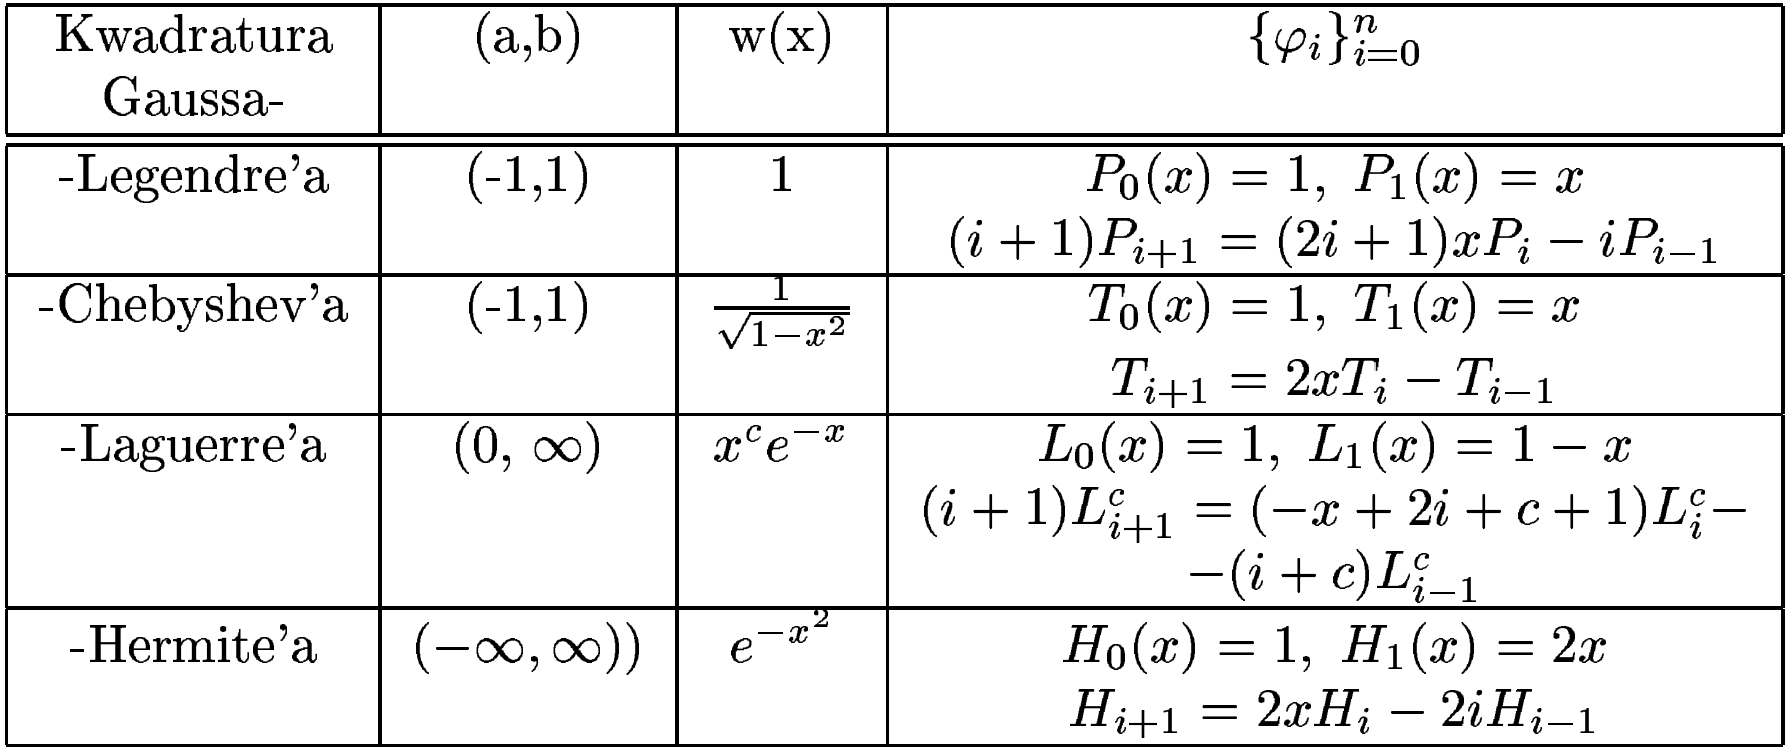
\includegraphics[width=.95\linewidth]{img/6/6_03}
		\end{figure}
  \end{frame}


























